\documentclass[a4paper]{scrartcl}%{{{
\usepackage{float}
\usepackage{tikz}
\usetikzlibrary{arrows,automata}
\usepackage{pgf}
\usepackage[utf8x]{inputenc} % this is needed for umlaut}s
\usepackage[ngerman]{babel} % this is needed for umlauts
\usepackage[T1,T5]{fontenc}    % this is needed for correct output of umlauts in pd
\usepackage{amssymb}
\usepackage{amsmath}
\usepackage{mathtools, nccmath}
\usepackage{mathabx}
\usepackage{mathrsfs}
\usepackage{dsfont}
\usepackage{wasysym}
\usepackage{graphicx}
\usepackage{fancyhdr}
\usepackage{lastpage}
\usepackage{imakeidx}
\setlength{\parskip}{\medskipamount}
\setlength{\parindent}{0pt}
\usepackage{enumitem}
\usepackage{hyperref}
\usepackage{verbatim}

%%%%%%%%%%%%%%%%%%%%%%%%
% Kopf- und Fusszeilen %
%%%%%%%%%%%%%%%%%%%%%%%%
\pagestyle{fancy}
\lhead{
        Maximilian Roth:
}
\chead{Phong Illumination Model}
\rhead{
    \begin{tabular}{rr}
        \today{} \\
        Seite \thepage{} von \pageref{LastPage}
    \end{tabular}
}
\lfoot{}
\cfoot{}
\rfoot{} 

\title{Phong Illumination Model}
\author{Maximilian Christian Roth}


%%%%%%%%%%%%%%%%%%%%%%%%
% Anfang des Dokuments %
%%%%%%%%%%%%%%%%%%%%%%%%%
\begin{document}
%}}}

\maketitle
\tableofcontents

\newpage

\section{Einführung}%{{{
\label{sec:einfuhrung}

    Das Phong-Illumination-Model oder Phong Beleuchtungsmodell ist ein Verfahren zur Berechnung der Intensität von Reflexionen auf der Oberfläche von Objekten,\\
    welches im Jahr 1975 von Bùi Tường Phong \footnotemark[1] vorgestellt wurde.\\
    \footnotetext[1]{Bùi Tường Phong: \url{https://en.wikipedia.org/wiki/Bui_Tuong_Phong}} %}}}

\section{Inputs \& Outputs}%{{{
\label{sec:inputs_outputs}

    Um die Reflexion für einen Punkt zu berechnen benötigen wir einige Hintergrundinformationen:\\
    \begin{table}[H]
    \caption{Wichtige Notationen}
    \label{table:vars}
    \begin{tabular}{l|l|l}
        \hline
        \multicolumn{1}{|c|}{Variable} & \multicolumn{1}{c|}{Bedeutung}                         & \multicolumn{1}{c|}{Typ} \\ \hline
        $\vec{P}$                              & Der betrachtete Punkt auf der Oberfläche eines Objekts & Vektor                   \\ \hline
        $\vec{N}$                              & Die Oberflächennormale des Punktes                     & Vektor                   \\ \hline
        $\vec{L}$                              & Der Vektor von P zur Lichtquelle                       & Vektor                   \\ \hline
        $\vec{R}$                              & Der reflektierte Lichtvektor am Punkt P                & Vektor                   \\ \hline
        $\vec{V}$                              & Der Vektor von P zum Viewpoint                         & Vektor                   \\ \hline
        $[I_{a}]$                    & Die Intensität des Umgebungslicht                      & RGB-Vektor               \\ \hline
        $[I_{in}]$                         & Die Intensität einer Lichtquelle                       & RGB-Vektor               \\ \hline
        $[I_{ambient}]$                         & Die Intensität der ambienten Lichtreflexion                       & RGB-Vektor               \\ \hline
        $[I_{diffus}]$                         & Die Intensität der diffusen Lichtreflexion                       & RGB-Vektor               \\ \hline
        $[I_{spekular}]$                         & Die Intensität der spekularen Lichtreflexion                       & RGB-Vektor               \\ \hline
        $[k_{ambient}]$                    & Die ambiente Materialkonstante                         & RGB-Vektor               \\ \hline
        $[k_{diffus}]$                     & Die diffuse Materialkonstante                          & RGB-Vektor               \\ \hline
        $[k_{spekular}]$                   & Die spekulare Materialkonstante                        & RGB-Vektor              \\ \hline
        n                   & Die Rauigkeit des Materials                        & Konstante              \\ \hline
        m                   & 'Shininess' im Blinn-Phong-Model                        & Konstante
    \end{tabular}
    \end{table}

    \begin{figure}[H]
        \centering
        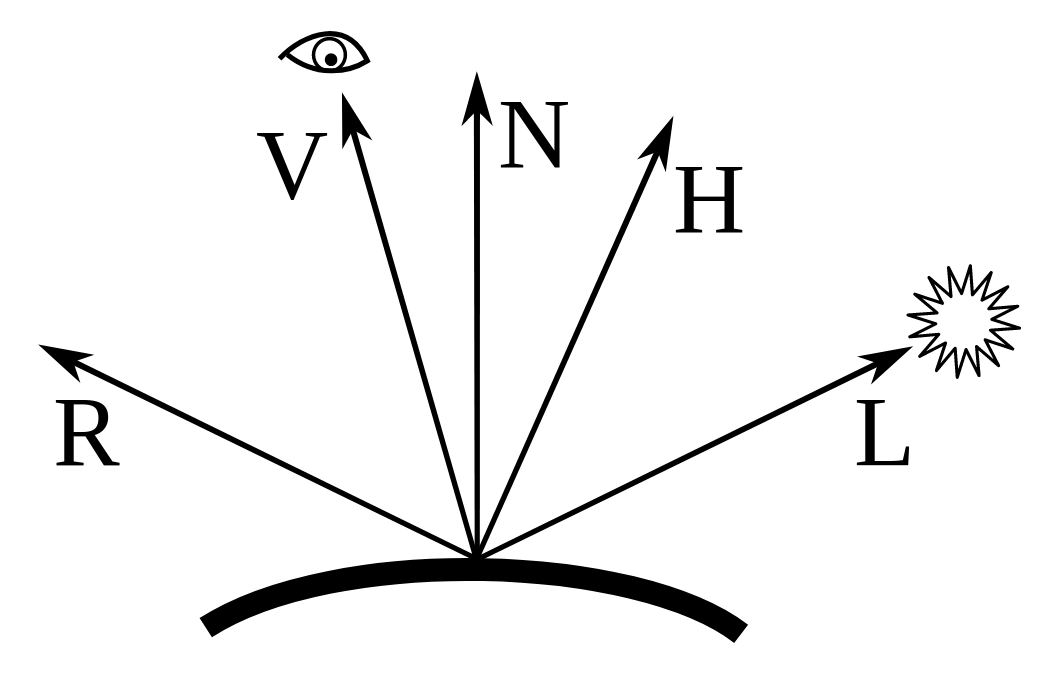
\includegraphics[scale=0.3]{./possible-images/Diagram.png}
        \caption{Veranschaulichung einiger Variablen [1]}
        \label{fig:./possible-images/Diagram}
    \end{figure}
    %}}}


\section{RGB-Vektoren}%{{{
\label{sec:rgb_vektoren}
    In der Computergraphik werden verschiedene Werte, wie zum Beispiel - bei üblichen Implementationen des Phong-Illumination-Models -
    die Intensität von Licht und Materialkonstanten, die etwas über das Reflexionsverhalten eines Objekts aussagen, als RGB-Vektoren dargestellt.\\
    Diese RGB-Vektoren sind in drei Kompontenten aufgeteilt, welche sind:\\
    \\\centerline{[v] = [rot, grün, blau]}\\
    \\Das heißt jeder Punkt eines Objektes wird durch die drei Farbkomponenten rot, grün und blau in seiner Farbe und Farbhelligkeit beschrieben.\\
    Die Werte für die Komponenten sind dabei Integer im Intervall von [0,255].\\
    Solche Vektoren haben besondere Berechnungsvorschriften:\\
    \\Seien [x], [y] RGB-Vektoren und c eine Konstante
    
    \subsection{Addition von RGB-Vektoren}%
    \label{sub:addition_zweier_rgb_vektoren}
        Die Addition von zwei RGB-Vektoren ist wie die von normalen Vektoren Kompontentenweise.\\
        \begin{equation}
            \label{eq:rgb-add}
            [x] + [y] =  [x_r + y_r, x_g + y_g, x_b + y_b]\\
        \end{equation}
     
    \subsection{Multiplikation von RGB-Vektoren}%
    \label{sub:multiplikation_von_rgb_vektoren}
        Die Multiplikation zweier RGB-Vektoren ist ebenfalls Kompontentenweise.\\
        \begin{equation}
            \label{eq:rgb-mult}
            [x] \cdot [y] = [x_r \cdot y_r, x_g \cdot y_g, x_b \cdot y_b] 
        \end{equation}

    \subsection{Multiplikation eines RGB-Vektors mit einer Konstante}%
    \label{sub:multiplikation_eines_rgb_vektors_mit_einer_konstante}
    
        Die Multiplikation eines RGB-Vektors mit einer Konstante:\\
        \begin{equation}
            \label{eq:rgb-const}
            [x] \cdot c = [x_r \cdot c, x_g \cdot c, x_b \cdot c]\\
        \end{equation}%}}}
    

\section{Phongs Reflexionstypen}%
\label{sec:phongs_reflexionstypen}

    Im Phong-Illumination-Model \footnotemark[2] unterscheidet Bùi Tường Phong bei der Berechnung die Reflexion von Licht in folgende drei Subtypen:\\
    \footnotetext[2]{Paper: \url{http://www.cs.northwestern.edu/~ago820/cs395/Papers/Phong_1975.pdf}}

    \subsection{Die ambiente Reflexion}%{{{
    \label{sub:die_ambiente_reflexion}
        Das Umgebungslicht, das von anderen Objekten im Raum and den betrachteten Punkt P (Siehe Tabelle ~\ref{table:vars}) reflektiert wird.\\
        Physikalisch gesehen müsste hier für jeden Punkt der Weg jedes Photons berechnet werden, um eine realistische Reflexion zu erreichen.\\
        Da dies jedoch sehr auswändig wäre wird einfach eine Umgebungslichtintensität für den Punkt gegeben mit dem dann die Reflexion berechnet wird.\\
        Die meisten Implementationen des Phong-Illumination-Models machen es sich jedoch noch einfacher und nehmen global die selbe Intensität an.\\
        \\Berechnet wird die Intensität der Reflexion des ambienten Lichts in der Regel wie folgt:\\
        \begin{equation}
            \label{eq:amb}
                [I_{ambient}] = [I_a] \cdot [k_{ambient}]\\
        \end{equation}
        Für die Variablen siehe Tabelle ~\ref{table:vars}\\

        \begin{figure}[H]
            \centering
            
\includegraphics[scale=0.2]{./possible-images/light-types/ambient.jpg}
            \caption{Figur mit rein ambienter Reflexion}
            \label{fig:./possible-images/light-types/ambient}
        \end{figure}%}}}

    \subsection{Die diffuse Reflexion}%{{{
    \label{sub:die_diffuse_reflexion}
        Der zweite Typ, in den Phong Reflexion unterteilt ist die diffuse Reflexion.\\
        Sie beschreibt, wie Licht, das direkt von einer Lichtquelle auf das Objekt trifft absorbiert, und damit auch wie es reflektiert wird.\\
        Hier wird das von anderen Objekten auf den betrachteten Punkt reflektierte Licht nicht betrachtet.\\
        \\Die Berechnungsvorschrift lautet:\\
        \begin{equation}
            \label{eq:diff}
            \begin{multlined}[b]
                [I_{diffus}] = [I_{in}] \cdot [k_{diffus}] \cdot cos(\Phi)\\
                \overset{(*)}{=} [I_{in}] \cdot [k_{diffus}] \cdot <\vec{L}, \vec{N}>\\
            \end{multlined} 
        \end{equation}
        Für die Variablen siehe Tabelle ~\ref{table:vars}\\

        (*): Nur, wenn die Vektoren im Skalarprodukt normalisiert sind, da folgende Gleichung gilt:\\
        \begin{equation}
            \label{eq:dot-prod}
            <\vec{a}, \vec{b}> = ||\vec{a}|| \cdot ||\vec{b}|| \cdot cos(\gamma)
        \end{equation}
        \centerline{Wobei $\gamma$ der Winkel zwischen $\vec{a}$ und $\vec{b}$ ist.}\\
        
        \begin{figure}[H]
            \centering
            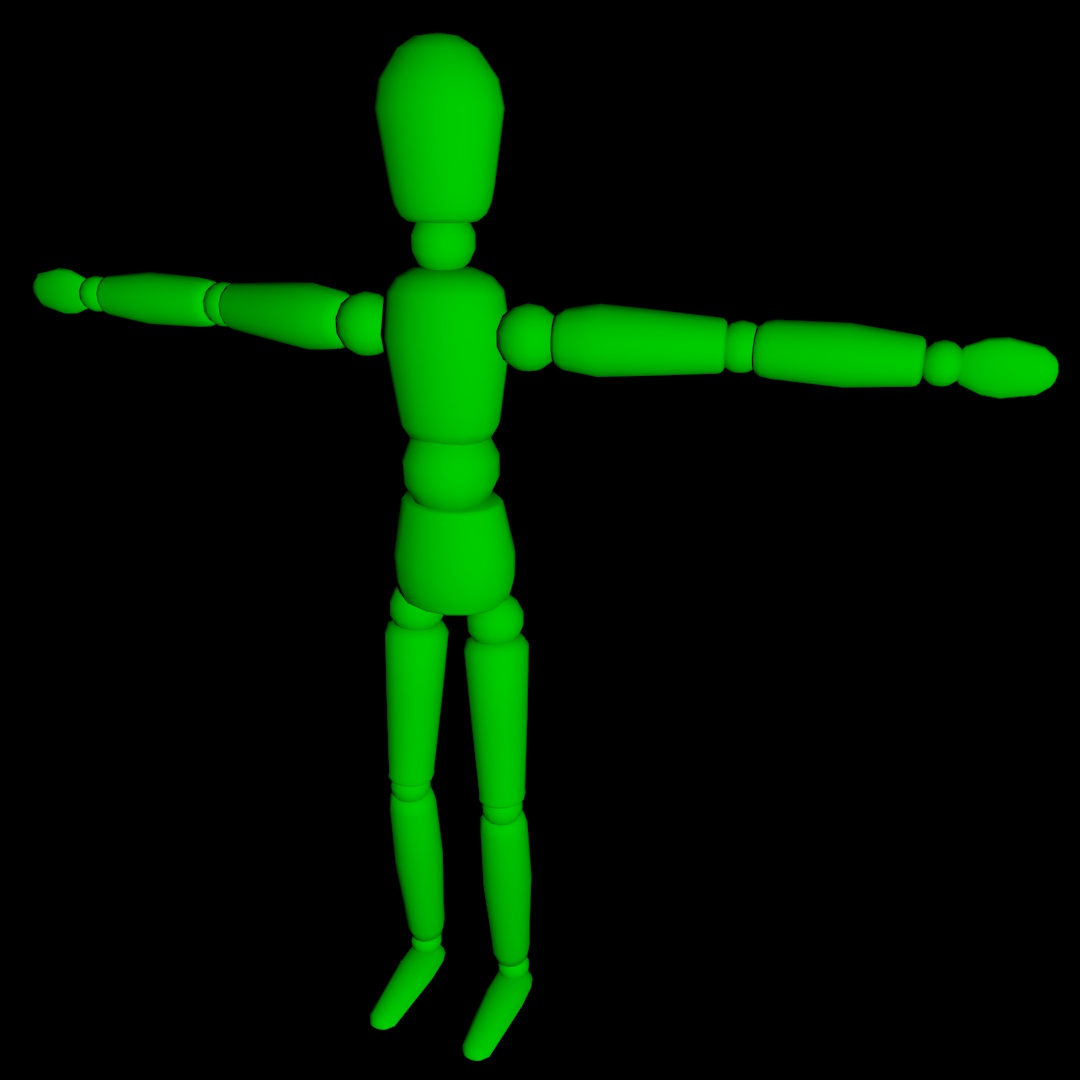
\includegraphics[scale=0.2]{./possible-images/light-types/diff.jpg}
            \caption{Figur mit rein diffuser Reflexion}
            \label{fig:./possible-images/light-types/diff}
        \end{figure}
         
        %}}}

    \subsection{Die spekulare Reflexion}%{{{
    \label{sub:die_spekulare_reflexion}
        Der dritte und letzte Typ, in welchen Phong das Licht unterteilt ist das spekulare Licht. Dieser Teil ist die Glanzreflexion des Lichtes.\\ \\Die Intensität der Glanzreflexion hängt natürlich vom Material am Punkt ab (ein Spiegel reflektiert viel mehr, als Beispielsweise ein Stück Holz).
        Ebenso ist die Position\\ des Lichtes wichtig, denn je nachdem wo die Lichtquelle sich befindet wird auch\\ in eine andere Richtung reflektiert.
        Weiters ist auch die Position des Betrachters,\\ also der Viewpoint wichtig, da relevant ist, ob das Licht in seine Richtung reflektiert wird oder an ihm vorbei.\
        \\Folgende Formel dient zur Berechnung:\\
        
        \begin{equation}
            \label{eq:spek}
            \begin{multlined}[b]
                [I_{spekular}] = [I_{in}] \cdot [k_{spekular}] \cdot cos^n(\Theta)\\
                \overset{(*)}{=} [I_{in}] \cdot [k_{spekular}] \cdot <\vec{R}, \vec{V}>^n\\
            \end{multlined} 
        \end{equation}
    
         
        Für die Variablen siehe Tabelle ~\ref{table:vars}\\
        
        \begin{figure}[H]
            \centering
            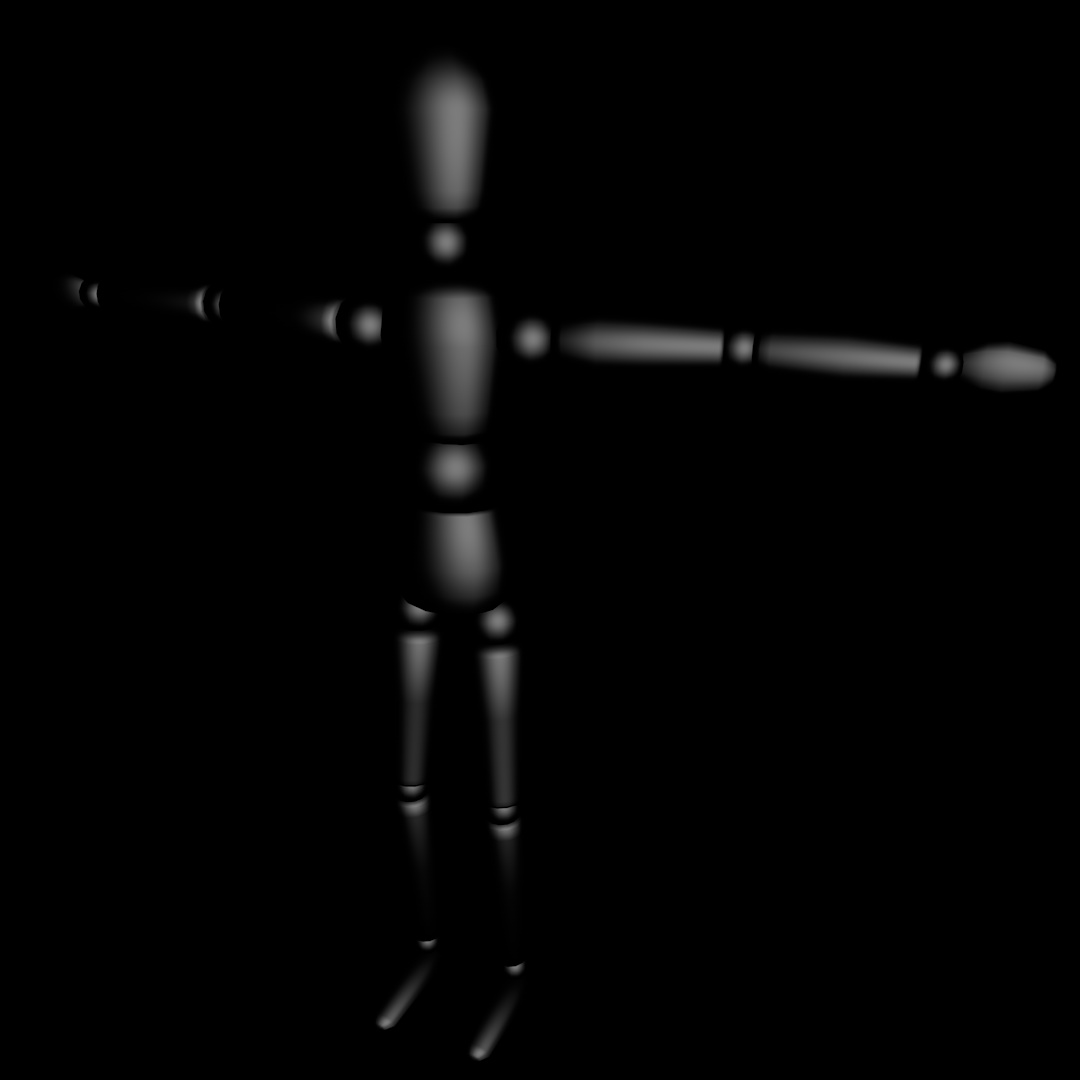
\includegraphics[scale=0.2]{./possible-images/light-types/spec.jpg}
            \caption{Figur mit rein spekularer Reflexion}
            \label{fig:./possible-images/light-types/spec}
        \end{figure}
        
        %}}}

    \subsection{Das gesamte Phong Beleuchtungsmodell}%{{{
    \label{sub:das_gesamte_phong_beleuchtungsmodell}
        Da die Unterteilung in diese drei Kompontenten in der Natur nicht existiert, sondern die Komponenten eigentlich Teil eines Physikalischen Phänomens sind und
        die Aufteilung nur der Vereinfachung der Berechnung dient müssen wir die Kompontenten wieder miteinander verrechnen.\\
        Dies geschieht in Phongs Beleuchtungsmodell durch simple Addition wie folgt:\\

        \begin{equation}
            \label{eq:phong}
            \begin{multlined}
                [I_{Phong}] = [I_{ambient}] + [I_{diffus}] + [I_{spekular}]\\
                = [I_a] \cdot [k_{ambient}] + [I_{in}] \cdot [k_{diffus}] \cdot cos(\Phi) + [I_{in}] \cdot [k_{spekular}] \cdot cos^n(\Theta)\\
                \overset{(*)}{=} [I_a] \cdot [k_{ambient}] + [I_{in}] \cdot ([k_{diffus}] \cdot <\vec{L}, \vec{N}> + [k_{spekular}] \cdot <\vec{R}, \vec{V}>^n)\\
            \end{multlined}
        \end{equation}

        Mit mehreren Lichtquellen $[I_{in}]_{1\leq i \leq k}$ ist $[I_{Phong}]$ die Summe der einzelnen Lichtquellen:\\
    
        \begin{equation}
            \label{eq:phong-multi}
            \begin{multlined}
                [I_{Phong}] = [I_{ambient}] + [I_{diffus}] + [I_{spekular}]\\
                = [I_a] \cdot [k_{ambient}] + \sum_k \Big([I_{in}]_k \cdot [k_{diffus}] \cdot cos(\Phi) + [I_{in}]_k \cdot [k_{spekular}] \cdot cos^n(\Theta)\Big)\\
                \overset{(*)}{=} [I_a] \cdot [k_{ambient}] + \sum_k \Big([I_{in}]_k \cdot ([k_{diffus}] \cdot <\vec{L}, \vec{N}> + [k_{spekular}] \cdot <\vec{R}, \vec{V}>^n)\Big)\\
            \end{multlined}
        \end{equation}
        
        \begin{figure}[H]
            \centering
            
\includegraphics[scale=0.2]{./possible-images/light-types/all.jpg}
            \caption{Figur mit allen drei von Phong unterschiedenen Reflexionstypen}
            \label{fig:./possible-images/light-types/all}
        \end{figure}
        
        %}}}
    
\section{Annahmen des Phong Modells}%{{{
\label{sec:annahmen_des_phong_modells}
    Das Phong-Illumination-Model trifft einige Annahmen, die in der Realität oder auch in unseren Simulationen möglicherweise nicht zutreffen:\\

    \subsection{Annahmen des Modells}%
    \label{sub:annahmen_des_modells}
    
        \begin{itemize}
            \item Alle Lichtquellen sind Punktförmig:\\
                Dies ist in der Realität nicht vorhanden, da alle Lichtquellen, die wir produzieren zwangsläufig dreidimensional sind.\\
            \item Für die Geometrie sind nur die Normalen relevant\\
        \end{itemize}
    
\newpage

    \subsection{Annahmen vieler Implementationen}%
    \label{sub:annahmen_vieler_implementationen}
    
        Weiterhin wird in den meisten Implementationen von folgendem augegangen:\\
        \begin{itemize}
            \item Reflexionen wirken sich nur ambient aus\\
                Offensichtlich jedoch müssen beispielsweise Spiegel das von anderen Objekten reflektierte Licht jedoch selbst wieder spiegeln.\\
            \item Das ambiente Licht ist überall gleichstark:\\
                In der Realität ist an einem Lichtundurchlässigen Ort natürlich das Licht nicht gleich hell, wie an einem von Licht leicht erreichbarem Ort.\\
            \item Es kann mehr Licht von einem Punkt reflektiert werden, als auf ihn eintrifft:\\
                Widerspricht dem Energieerhaltungssatz der Physik.\\
        \end{itemize}
        Die zweite Annahme lässt sich dabei auf die erste zurückzuführen.\\
        Es stimmt jedoch nicht wie vielfach behauptet \footnotemark[3] \footnotemark[4] \footnotemark[5], dass dies Eigenschaften des Phong-Illumination-Models sind,
        da sie nicht in Phongs wissenschaftlichem Artikel stehen und unter Beachtung seines Modells behoben werden können.\\%}}}
        \footnotetext[3]{'diffuse und spiegelnde Reflexion wird nur lokal modelliert', 
        Quelle: \href{https://de.wikipedia.org/wiki/Phong-Beleuchtungsmodell}{Wikipedia} am 04.02.2019} 
        \footnotetext[4]{'ambiente Reflexion wird global modelliert', Quelle: \href{https://de.wikipedia.org/wiki/Phong-Beleuchtungsmodell}{Wikipedia} am 04.02.2019}
        \footnotetext[5]{'Es handelt sich um ein vollständig empirisches Modell, das auf keinerlei physikalischer Grundlage aufbaut.
        Das bedeutet, dass es dem Energieerhaltungssatz widerspricht', Quelle: \href{https://de.wikipedia.org/wiki/Phong-Beleuchtungsmodell}{Wikipedia} am 04.02.2019}

\newpage

\section{Quellen}%{{{
\label{sec:quellen}

    \subsection{Textquellen}%
    \label{sub:textquellen}
    
        \begin{itemize}
            \item \url{http://www.cs.northwestern.edu/~ago820/cs395/Papers/Phong_1975.pdf} 
            \item \url{https://cg.informatik.uni-freiburg.de/course_notes/graphics_04_lighting.pdf} 
            \item \url{https://en.wikipedia.org/wiki/Phong_reflection_model} 
            \item \url{https://de.wikipedia.org/wiki/Phong-Beleuchtungsmodell} 
            \item \url{http://www.mathematik.uni-marburg.de/~thormae/lectures/graphics1/code/WebGLShaderLightMat/ShaderLightMat.html} 
            \item \url{https://www.wikilectures.eu/w/Lambert%27s_law} 
            \item \url{https://en.wikipedia.org/wiki/Lambert%27s_cosine_law} 
            \item \url{https://wiki.delphigl.com/index.php/Beleuchtung} 
            \item \url{http://www.mathematik.uni-marburg.de/~thormae/lectures/graphics1/code/WebGLShaderLightMat/ShaderLightMat.html} 
        \end{itemize}

    \subsection{Bildquellen}%
    \label{sub:bildquellen}
    
        \begin{itemize}
            \item \url{https://en.wikipedia.org/wiki/File:Blinn_Vectors.svg}
            \item Die Bilder der Figuren sind selbst erstellt
        \end{itemize} %}}}


\end{document}
